\chapter{Estado da Arte - Teoria de Filas de Espera}
\label{cha:estadoDaArte}

Neste capítulo é apresentado o enquadramento sobre a teoria de filas de espera, de forma a expor todos os conceitos que podem ser utilizados para alcançar o objetivo principal do projeto. 

A ocorrência de filas de espera é um fenómeno do quotidiano, seja em lojas, no banco ou qualquer local onde é necessário esperar por um serviço. Atualmente, estamos habituados a um tempo de espera razoável nas filas. No entanto, sempre que este é maior que o normal, existem consequências que podem afetar por exemplo a economia de uma país visto que quanto maior tempo de espera, menor fornecimento de serviço existe.
A fila de espera é composta por duas componentes importantes, cliente e serviço.

Agner Krarkup Erlang (Lonborg, 1 de Janeiro de 1878 - Lonborg, 3 de Fevereiro de 1929) foi o matemático, estatístico e engenheiro dinamarquês que inventou os campos de Engenharia de Tráfego e da Teoria das Filas. A teoria das filas \cite{filasdeespera} \cite{operationsresearch}, é o estudo todas as diferentes filas de espera, utilizando modelos matemáticos para demonstrar o seu comportamento conforma a procura aleatória de clientes. Aplicando métricas aos modelos, tenta-se fornecer um atendimento adequado às necessidades dos clientes, indicando como é que a fila deve funcionar. 

As filas de espera são uma necessidade, visto que por norma, o número de clientes é superior ao número de servidores. 
O objetivo da teoria das filas de espera passa por otimizar o desempenho de um sistema, de modo a reduzir os seus custos operacionais e a aumentar a satisfação dos clientes. 

A existência de longas filas de espera em diversos tipos de serviço, constitui um problema que deriva do estabelecimento de \textit{trade-offs} entre o custo do serviço e o custo do tempo perdido pelos clientes na fila de espera.

\begin{figure}[ht]
	\centering
	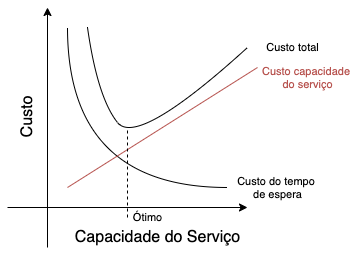
\includegraphics[width=0.85\textwidth]{tradeoff}
	  \caption{Trade-off entre o custo da capacidade do serviço e o custo do tempo de espera (retirada de Waiting Line Management: Costs Function and Service Level \cite{wlm})}
  \label{fig:trade_off}
\end{figure}

As filas de espera existem muito por causa da insuficiente capacidade dos serviços, que por sua vez, existe devido ao custo elevado a considerar pelo aumento da mesma. Por outro lado, o \textit{trade-off} representado na \figurename~\ref{fig:trade_off}, nem sempre é considerado, visto que só é avaliado o custo do serviço, o que diminui a capacidade de serviço, criando filas de espera.


\section{Sistema de fila de espera} 
\label{sec:sistemadefiladeespera}

\begin{figure}[ht]
    \centering
    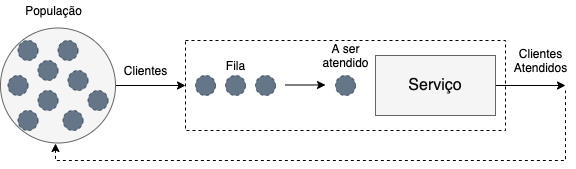
\includegraphics[width=0.85\textwidth]{temp/sistemadeiladeespera}
      \caption{Sistema de filas de espera (retirada de Filas de espera \cite{filasdeespera})}
  \label{fig:sistemadeiladeespera}
\end{figure}

Um sistema de filas, representado na \figurename~\ref{fig:sistemadeiladeespera}, é estruturada pelos clientes (população ou fonte), filas e pelo serviço de atendimento. O processo do sistema, dá-se início com os clientes a entrarem no sistema, juntando-se à fila pretendida (caso não esteja vazio), aguardando ser chamado pelo servidor, de acordo com uma regra, denominada por disciplina da fila. O cliente ao ser atendido, sai do sistema, podendo regressar posteriormente. Grande parte dos modelos de filas de espera utilizam este processo.

\begin{center} \textbf{Fila + Serviço = Sistema} \end{center} 
\begin{center} Número de clientes no sistema (em cada instante) = \textbf{estado do sistema} \end{center} 

\subsection{População ou Fonte} 

A população ou fonte é responsável por gerar os clientes que vão chegar ao sistema. Uma das características da fonte, é a dimensão, sendo o total de clientes que podem querer o serviço. Esta dimensão pode-se assumir como infinita/ilimitada ou finita/limitada. De forma a realizar os cálculos da previsão de tempo para as filas de espera, a dimensão da fila, não tem grande influência, visto que é necessário os tempos dos clientes já atendidos. A dimensão só irá servir para indicar a quantos clientes é que deve ser dado uma previsão. 

A chegada de clientes no sistema, é um aspeto importante na teoria de filas de espera, quando é pretendido lidar com análises das filas nos serviços. Essa chegada é indeterminada, podendo ter vários padrões distintos. Dessa forma é comum assumir que a chegada de clientes, tem uma distribuição de Poisson \cite{poissondistribuition}. Neste projeto não existe a necessidade de análise das chegadas, visto que o maior foco é os clientes já atendidos. \\

\subsection{Fila de espera} 

A fila de espera é onde os clientes ficam à espera de serem atendidos. Ela é caracterizada pelo número máximo de clientes que pode ter e disciplina da fila.

Relativamente ao número de filas, representado na \figurename~\ref{fig:filasunicasmultiplas}, pode-se considerar uma fila simples (fila única), onde pode haver um ou mais postos de atendimento (múltiplos servidores), ou múltiplas filas, com uma fila por posto de atendimento, onde cada par fila/posto de atendimento constitui um sistema separado de fila de espera.

\begin{figure}[ht]
    \centering
    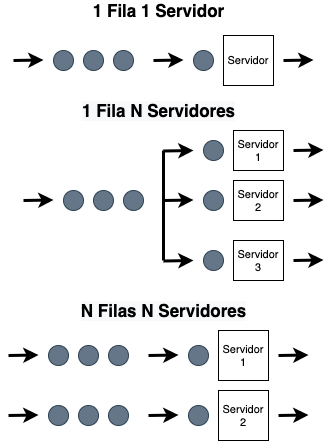
\includegraphics[scale=0.7]{temp/filasunicasmultiplas_new}
      \caption{Filas Únicas e Múltiplas (adaptado de Teoria das Filas \cite{teoriadasfilas})}
  \label{fig:filasunicasmultiplas}
\end{figure}

O comprimento da fila está relacionado com a capacidade do sistema, podendo ser finita de acordo com a limitação do espaço, ou pode infinita, quando não existe uma limitação ao tamanho da fila de espera.

Na \figurename~\ref{fig:filasunicasmultiplas}, é possível verificar os múltiplos tipos de servidores.

\subsection{Disciplina da fila de espera} 

A disciplina da fila de espera, se refere à ordem que os membros de uma fila são escolhidos para serem atendidos. Existem várias possibilidades, onde pode haver um atendimento por ordem de chegada ou por prioridade. A disciplina foco deste projeto é o atendimento por ordem de chegada, sendo uma disciplina \textit{\acrfull{fifo}}, conhecido também por \textit{\acrfull{fcfs}}. Esta disciplina, sendo a mais comum é a única considerada, visto que com o atendimento aleatória não é possível fornecer uma previsão sobre o tempo de espera aos clientes. Atendimentos por prioridade, pode ser inserido na disciplina \acrshort{fifo}, visto que geralmente existe uma fila própria que utiliza as mesmas regras.

\subsection{Serviço} 
O serviço corresponde aos postos onde os clientes podem obter/requerer serviços, em que cada contém canais paralelos de atendimentos, chamados servidores. A capacidade de cada posto, é determinada pelo número de canais paralelos disponíveis e pela capacidade de cada canal em servir os clientes. Esta componente do sistema, tem grande importância, tendo em conta a tamanha influência que pode ter no tempo despendido pelos clientes nos postos de serviço e na economia do serviço.


\subsection{Medidas de desempenho}

De forma a gerir um sistema de filas de espera algumas medidas têm que ser levadas em conta:

\begin{itemize}
\item Comprimento médio da fila
\item Número médio de clientes no sistema
\item Tempo médio de espera na fila
\item Tempo médio de espera no sistema
\item Taxa média de ocupação do serviço
\end{itemize}

Com essas medidas é possível encontrar soluções equilibradas que permitem estabelecer \textit{trade-offs} entre custo e qualidade de serviço.

\begin{figure}[ht]
    \centering
    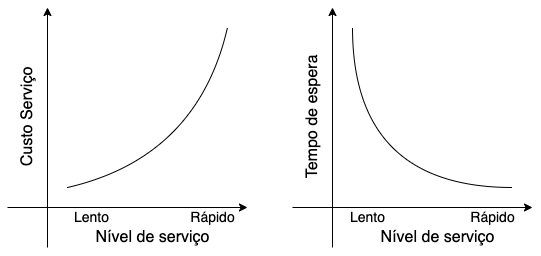
\includegraphics[width=0.85\textwidth]{funcoestempoespera}
      \caption{Funções de custo de serviço e tempo de espera em relação ao nível do serviço (adaptada de Waiting Line Management: Costs Function and Service Level \cite{wlm})}
  \label{fig:funcoestempoespera}
\end{figure}

Na \figurename~\ref{fig:funcoestempoespera}, é possível observar que quanto maior o nível do serviço, menor o tempo de espera, tendo no entanto um custo bastante acrescido à medida que esse nível aumenta.


\section{Processo de vida e morte}
No contexto do sistema de filas de espera, em grande parte do modelos de filas elementares, assume-se que a chegada de clientes à fila e a consequente saída, ocorre de acordo com o processo de vida e morte. A este processo, vida (nascimento) se refere à entrada enquanto que morte é a saída de um cliente já atendido (\figurename~\ref{fig:processovidamorte}). A modelização deste processo, supõe estados de equilíbrio, excluindo por exemplo a variação da taxa de chegada, ou a possibilidade de ter números anormais de clientes no início do funcionamento. Neste processo, assume-se as seguintes hipóteses:

\begin{itemize}
        \item Dado o instante t, com o sistema no estado n:
        \begin{itemize}
        \item A probabilidade do próximo nascimento (chegada) segue uma distribuição exponencial negativa com parâmetro $\lambda$n;
        \item A probabilidade próxima morte (serviço terminado) segue uma distribuição exponencial negativa com parâmetro $\mu$n.
        \end{itemize}
    \item Nunca podem ocorrer simultaneamente mais do que um nascimento ou uma morte.
\end{itemize}

\begin{figure}[ht]
    \centering
    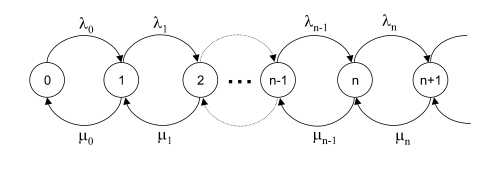
\includegraphics[width=0.85\textwidth]{processovidamorte}
      \caption{Diagrama de transição correspondente ao processo de vida e morte (retirada de Filas de espera \cite{filasdeespera})}
  \label{fig:processovidamorte}
\end{figure}

\section{Modelos das filas de espera baseados nos processos de vida e morte} 
A maioria dos modelos analíticos de filas de espera, têm como base o processo de vida e morte, onde as entradas têm uma distribuição de Poisson \cite{poissondistribuition} e tempos de atendimento com distribuição exponencial negativa. No entanto, cada modelo se difere nas suas assumpções sobre como é que a chegada e a saída afetam o estado do sistema. 

\subsection{Classificação da filas de espera - X/Y/Z/W}
X, Y — Distribuições do intervalo de tempo entre chegadas e do tempo de serviço,
respetivamente:
\begin{itemize}
\item M — distribuição exponencial negativa
\item G — distribuição não especificada
\item D - chegadas ou atendimentos determinísticos
\end{itemize}
Z — número de servidores em paralelo.

W — outras características do sistema, tais como comprimento da fila ilimitado ou população finita:
\begin{itemize}
\item em branco ou $\infty$ — modelo-base sem qualquer restrição adicional
\item K — comprimento da fila limitado, não podendo o número de elementos no
sistema exceder K
\item N - população finita
\end{itemize}


\subsection{Modelo M/M/1}

Neste modelo, existe um único posto de atendimento (1) e assume-se que a distribuição do intervalo de tempo entre chegadas (M) e do tempo de serviço (M) é exponencial. Assume-se que o sistema tem capacidade ilimitada, e população, utilizando uma disciplina \acrshort{fifo}/\acrshort{fcfs} no atendimento.

\subsection{Modelo M/M/S}
Neste modelo, existem múltiplos servidores (S), que fornecem serviço independentemente uns dos outros. Assume-se que a distribuição do intervalo de tempo entre chegadas (M) e do tempo de serviço (M) é exponencial. Assume-se que o sistema tem capacidade ilimitada, e população, utilizando uma disciplina \acrshort{fifo}/\acrshort{fcfs} no atendimento.

\subsection{Modelo M/M/1/K}
Este modelo difere de M/M/1 visto que tem a capacidade do sistema limitada até K clientes ao mesmo tempo no local de prestação de serviço. Quando o sistema tiver K clientes, será recusado novas chegadas de cliente. A disciplina utilizada é a \acrshort{fifo}.

\subsection{Modelo M/M/S/K}
Neste modelo, o sistema tem capacidade finita, com s servidores, com tempos de atendimento exponenciais independentes e identicamente distribuídos (não dependem do estado do sistema). A capacidade do sistema deve ser, no mínimo, tão grande quanto o número de servidores, K $\geqslant$ s. Utiliza a disciplina \acrshort{fifo}.

\subsection{Modelo M/M/$\infty$}
Neste modelo, o serviço é ilimitado, existindo um número infinito de servidores disponíveis, não existindo uma fila de espera. A distribuição do intervalo de tempo entre chegadas e tempo de serviço é exponencial. A capacidade do sistema e da população é infinita. A disciplina seguida é a \acrshort{fcfs}.

\subsection{Outros modelos}
Para a análise de filas de espera, existem vários tipos de modelos, no entanto neste trabalho só é tido em consideração os modelos com distribuição exponencial.

\section{Redes de filas de espera}
Em muitos casos reais, um cliente pode passar por uma sucessão de filas, provocando dessa forma um sistema com múltiplas fases, ficando perante uma rede de filas de espera. Um exemplo seria as urgências hospitalares, onde é necessário passar por uma fase de triagem até à consulta e a possíveis exames. 

\section{Considerações finais sobre filas de espera}
Em qualquer posto de serviço existente, vai sempre existir filas de espera para os clientes, em vários modelos diferentes. A criação de um sistema de gestão de senhas e de previsão de tempos de espera irá ter impacto na forma como os clientes são atendidos, permitindo a estes uma melhor gestão do tempo para outras tarefas enquanto aguardam a vez de ser atendido. Os dados recolhidos podem ajudar a otimizar a forma como cada serviço trabalha no dia-a-dia.
